\graphicspath{{Chapter-Experiment/figures/}}
\chapter{Experimental design and apparatus}
\section{Scattering experiments}

\subsection{History and motivation}
The first modern scattering experiment could be said to be the Geiger-Marsden experiments in the early 1910s, in which the Rutherford scattering of alpha ($\alpha$) particles by gold foil was observed \cite{Rutherford:1911zz}.
While most $\alpha$ particles pass through the foil with little deflection, a small fraction of them are deflected to extreme angles (\Fig{\ref{fig:rutherford}}).
This result provided evidence that electric charge within the foil was not distributed uniformly, but localized in very small clusters -- the nuclei of the gold atoms.
\begin{figure}[t]
  %% https://www.chegg.com/homework-help/questions-and-answers/rutherford-s-experiment-studied-deflection-scattering-ofalpha-particles-known-helium-nucle-q458296
  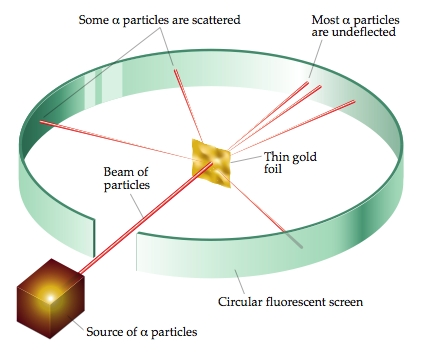
\includegraphics[width=0.8\linewidth]{BLB-1070873-Rutherford_v2.jpg}
  \caption{Rutherford scattering of alpha particles by gold foil, demonstrating the existence of the atomic nucleus.}
  \label{fig:rutherford}
\end{figure}

With elementary quantum mechanics, this type of elastic scattering can be understood a little more precisely.
In the Born approximation, which is essentially the weak-potential limit, the quantum amplitude $f$ of a particle with incoming momentum $\mathbf{p}_{i}$ scattering elastically off a target potential $V(\mathbf{x})$ with outgoing momentum $\mathbf{p}_{f}$ is proportional to the Fourier transform of the potential:

\begin{equation}
  f\left(\mathbf{p}_f ; \mathbf{p}_i\right) \propto - \int d^3 x \, V(\mathbf{x}) e^{-i \Delta \mathbf{p} \cdot \mathbf{x}}
  \label{eqn:born}
\end{equation}
where $\Delta \mathbf{p} \equiv \mathbf{p}_f - \mathbf{p}_i$ is the momentum transferred to the projectile particle.
The differential scattering cross section $d\sigma/d\Omega$ (the scattering probability density per unit area) is given by the square of the quantum amplitude, so it is proportional to the squared magnitude of the Fourier transform of the potential.

\begin{equation}
  \frac{d\sigma}{d\Omega} \propto \left| \int d^3 x \, V(\mathbf{x}) e^{-i \Delta \mathbf{p} \cdot \mathbf{x} / \hbar} \right|^2 = \left| \tilde{V}(\mathbf{\Delta \mathbf{p}}) \right|^2
\end{equation}
Because the net momentum transfer is constrained by the relative momentum between projectile and target, larger momentum -- or equivalently, higher energy -- is required to probe finer structure of the target.
This correspondence between center-of-mass energy and the spatial resolution of the probe remains valid even for inelastic collisions and strong interactions.
The required energy to probe a distance scale can be estimated with dimensional analysis.
To resolve the structure of a target down to a distance scale $l$, the center-of-mass energy $E$ is

\begin{equation}
E = \frac{\hbar c}{l} \approx \frac{0.2 \GeV \fm}{l} \; .
\end{equation}
Resolving individual atoms requires collisions with energy of order \keV, resolving the nucleus requires at least \MeV, and resolving sub-nucleic structure requires collisions of at least \GeV energies.

\subsection{Accelerator physics}

In a fixed-target experiment using target particles of mass $m_t$ at rest and a projectile beam with particles of mass $m_p$ and energy $E$, the center-of-momentum energy $\sqrt{s}$ is given by
\begin{equation}
\sqrt{s} = \sqrt{(m_t+m_p)^2 + 2 m_t (E - m_p)} \; ,
\end{equation}
which scales with the square root of the beam energy even for large energies.
On the other hand, if two beams are accelerated and directed into each other, the center-of-momentum energy of each collision is
\begin{equation}
\sqrt{s} = \sqrt{(E_t + E_p)^2 - (|\mathbf{p}_t| - |\mathbf{p}_p|)^2} \; ,
\end{equation}
which scales linearly with the total energy, and is equal to $2E$ in the case where the beams are identical.
While fixed-target experiments were the first to be developed, they are not as efficient at reaching high energies as dual-beam colliders.
Modern high-energy experiments therefore accelerate two particle beams and generate collisions by intersecting the beams head-on.

\subsubsection{Accelerator designs}

\begin{figure}[t]
  %%  https://www.cyberphysics.co.uk/topics/atomic/Accelerators/LINAC/Linac.htm
  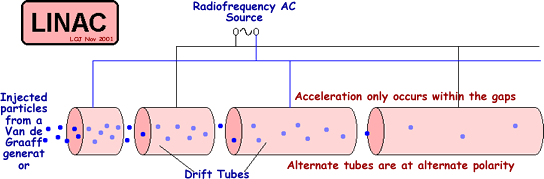
\includegraphics[width=0.8\linewidth]{LINAC.png}
  \caption{A linear accelerator.}
  \label{fig:linac}
\end{figure}

The most straightforward method to accelerate charged particles to high energies is to allow them to pass through a large voltage differential.
A large voltage can be produced, for instance, with a Van de Graaff generator \cite{PhysRev.43.149}.
The voltage differential is limited by the insulation breakdown, which in practice caps the energy of accelerated particles with charge $Ze$ to a few $Z \cdot\MeV$.
A modern linear particle accelerator (linac) circumvents this issue by passing ions through a series of drift tubes with alternating positive and negative potentials (\Fig{\ref{fig:linac}}).
The drift tubes are constructed with conducting material, so they shield the ions traveling through them from external electric acceleration.
Between the drift tubes, however, strong electric fields are induced by the alternating potentials.
This voltage difference is oscillated with radio frequency (RF) and the apparatus is constructed such that ions injected at a given velocity can pass through each gap with acceleration in the forward direction.
The Stanford Linear Accelerator Center (SLAC) hosts the largest linear accelerator, which began operation in 1966.
The 3 km long machine was capable of accelerating electrons and positrons to energies of up to 50 \GeV.
While this is several orders of magnitude higher than the energies accessible with simple voltage differential, increasing the energy further requires proportional increases to the length of the accelerator, exacerbating technical difficulties in its placement, construction, and maintenance.

\begin{figure}[t]
 %% https://www.mpoweruk.com/figs/cyclotron.htm
  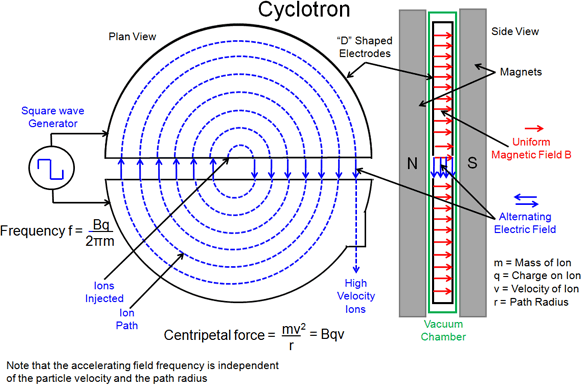
\includegraphics[width=0.8\linewidth]{cyclotron.png}
  \caption{A cyclotron.}
  \label{fig:cyclotron}
\end{figure}
The cyclotron is the next fundamental progression in accelerator technology.
Ions in a cyclotron are passed between two semi-cylindrical electrodes (``dees'') that are driven with an alternating voltage (\Fig{\ref{fig:cyclotron}}).
A large electromagnet keeps the particles traveling in a circular path contained within the dees.
At non-relativistic energies, the velocity of the ions is proportional to the radius of their path, so the time taken for one revolution is independent of the velocity.
If the voltage between the electrodes is oscillated with a frequency equal to the cyclotron resonance frequency $f_\textrm{cyclo} = q B / 2\pi m$, then ions are accelerated to higher energies with each pass between the dees.
At a fixed radius (and therefore fixed energy), the ion beam is allowed to exit the cyclotron.
Classically, the kinetic energy is proportional to the square of the radius, inviting a comparison to a hypothetically coiled linac.
Relativistic energies can be attained with more sophisticated designs that vary either the frequency over time or the magnetic field with the radial position, but as the velocity approaches $c$ the energy is only linearly proportional to the radius:
\begin{align}
\label{eqn:gyroradius}
E =& \; \frac{q B R c^2}{v}\\
\overrightarrow{{}_{v \rightarrow c}}& \; q B R c
\end{align}
This shows that the energies accessible from a circular accelerator are directly limited by the maximum strength of the magnetic field and the radius of the path.

The radius of a cyclotron design can only be increased so much before it becomes infeasible.
The synchrotron is a toroidal accelerator in which ion beams travel around the torus, turned by dipole magnets along the path.
Quadrupole and higher-multipole magnets are used to maintain the focus of the beam and make fine-tuning adjustments to the magnetic fields.
This layout does not permit it to accelerate particles from an arbitrarily small energy, so a synchrotron is generally filled with a linac first, with the ions circling the path at a constant energy.
Once the beam pipe is filled, the energy of the ion beam is gradually increased by RF cavities that oscillate to apply an acceleration to the particles.
The oscillation of the RF cavities groups the ions into bunches along the beam.
The limiting factor for synchrotron performance depends on the mass of the particle; for electrons the power lost via synchrotron radiation $P_\textrm{synch-rad} \propto e^2 E^4 / m^4 R^2 $ is the limiting factor in the maximum energy.

\subsubsection{Luminosity}

The capability of an accelerator to provide collision events to a detector is chacterized by its luminosity.
The rate of inelastic collisions $dN/dt$ is proprotional to the total inelastic cross-section of the collision participants $\sigma$.
The proportionality factor is defined as the \emph{instantaneous luminosity} $\mathcal{L}$.
\begin{equation}
\label{eqn:rate_lumi}
\frac{dN}{dt} = \sigma \mathcal{L}
\end{equation}
The total number of events is proportional to the \emph{total luminosity} $L = \int \mathcal{L} \, dt$.
\begin{equation}
N = \sigma L
\end{equation}
This definition is useful because it separates the contributions to the observations ($N$) into the independent contributions from physics ($\sigma$) and from the accelerator ($L$).

\section{The Large Hadron Collider}

The Large Hadron Collider (LHC) is a high-energy particle ring collider located near Geneva on the Swiss-French border \cite{LHCMachine}.
It was constructed by the European Organization for Nuclear Research (CERN, for ``Conseil européen pour la recherche nucléaire'') and is currently the highest energy particle accelerator in the world, with a design center-of-mass energy for proton collisions of \ppenergy.
Two adjacent beam pipes lay in a 26.7 km circumference, and are filled in anti-aligned orientation so that the beams can be crossed to generate collisions.
While it was primarily designed to provide proton-proton (\pp) collisions, it is also capable of colliding lead (${}^{208}_{\ 82}\textrm{Pb}$) and xenon (${}^{129}_{\ 54}\textrm{Xe}$) ions with themselves and with protons.
The results of this thesis will use data collected from the 2013 \pPb collisions, which were taken at a center-of-mass energy per nucleon of \pPbenergy.

\subsection{Injection chain}

\begin{figure}[t]
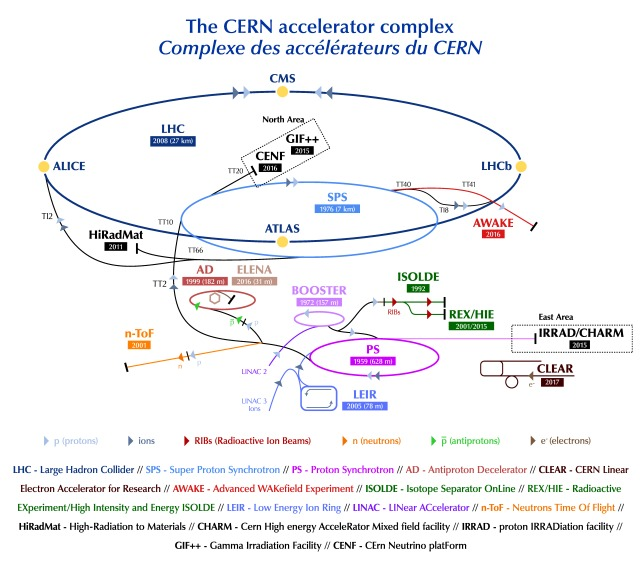
\includegraphics[width=0.8\linewidth]{CCC-v2018-print-v2.jpg}
\caption{The LHC is the last ring (dark blue line) in a complex chain of particle accelerators. The smaller machines are used in a chain to help boost the particles to their final energies and provide beams to a whole set of smaller experiments. (Copyright CERN \cite{Mobs:2636343})}
\label{fig:injection_chain}
\end{figure}

Before being injected into the LHC, ion beams pass through a series of increasingly large accelerators, incrementally raising their energy \cite{Benedikt:2004wm}.
These lower-energy accelerators predate the LHC and have each been used for many collision experiments throughout the history of CERN.
The CERN accelerator complex is sketched in \Fig{\ref{fig:injection_chain}}.

Protons are first collected by ionizing hydrogen gas, then accelerated to a kinetic energy of 50 \MeV by the Linac 2 linear accelerator.
The Proton Synchrotron Booster (PSB) increases their energy to the relativistic level of 1.4 \GeV.
From there, the beam is energized in the Proton Synchrotron (PS) to 25 \GeV, then the Super Proton Synchrotron (SPS) to 450 \GeV.
These proton beams from the SPS are used to fill the LHC, where they are again accelerated to collision energies of a few \TeV each.

Lead ions are accelerated from rest by the Linac 3 linear accelerator, a dedicated ion linac, to a kinetic energy of 4.2 \MeV per nucleon (\MeVn).
The Low Energy Ion Ring (LEIR) raises the energy to 72 \MeVn and also applies electron cooling to the ion beam.
This process involves merging the ions with an electron beam and allowing the mixture to come to thermal equilibrium, so that the electron cloud absorbs thermal energy from the ions.
The ions are then re-separated from the electrons as they pass through a dipole magnet.
This cooling step, which effectively reduces the phase space volume of each bunch, is necessary to counteract the higher charge of the ions pushing them apart. %% equivalently, reducing the ``emittance'' of the beam
From the LEIR the lead ion beam is injected into the PS, which raises its energy to 5.9 \GeVn, then the SPS, which raises it to 177 \GeVn.
Finally, the beam is injected into the LHC, where it is accelerated to a few \TeVn depending on the intended collision system.


\subsection{LHC main ring}

\begin{figure}[t]
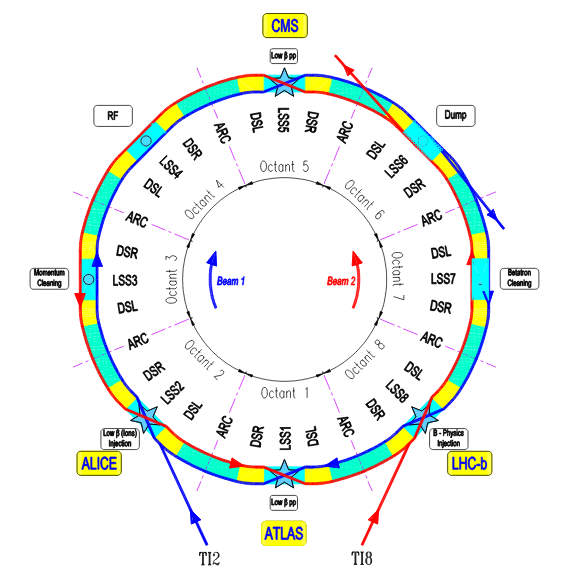
\includegraphics[width=0.8\linewidth]{LHC_schematic.png}
\caption{Schematic layout of the two beams of the LHC \cite{Bruning:2004ej}.}
\label{fig:lhc_schematic}
\end{figure}

The LHC ring does not trace a perfect circle, but is actually composed of eight alternating straight and curved arc sections (\Fig{\ref{lhc_schematic}}) \cite{Bruning:2004ej}.
Two parallel beam pipes 
The straight sections are each 528 m in length and carry the RF cavities for acceleration, interaction points for detector experiments, and other features like injection spots and beam dumps.
The arc portions have a radius of curvature of $R = 2.8$ km, using a total of 1232 superconducting dipole magnets to turn the beams along the path.

The RF cavities operate at 400 MHz, which corresponds to RF buckets of 2.5 ns.
For ultra-relativistic beams, this corresponds to a minimum length spacing between bunches of 0.75 m.
Practically, however, the injection from the SPS limits the bunch spacing to multiples of 25 ns, or 7.5 m separation.
The LHC can thus fit a maximum of 3560 bunches in each of its rings, but it is not completely filled because gaps need to be left to allow safe beam dumps.
The smallest bunch spacing used for lead ions is 150 ns.

\begin{figure}[t]
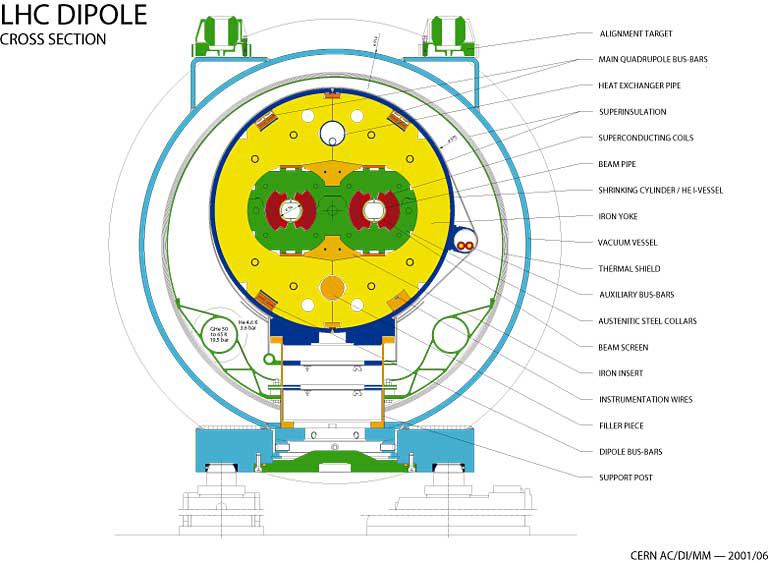
\includegraphics[width=0.8\linewidth]{LHC-PHO-2001-187.jpg}
\caption{A dipole magnet used to turn the beams along an arc. The two beams travel in the evacuated beam pipes running anti-parallel to each other, which requires the magnetic field in each to be opposite. (Copyright CERN \cite{Valeriane:843195})}
\label{fig:dipole_cross_section}
\end{figure}

The dipole magnets (\Fig{\ref{fig:dipole_cross_section}}) have a maximum design strength of 10 T, though the active field strength must remain proportional to the current energy of the beam fill.
For the \pPbenergy \pPb run they operated at 6.0 T with fully energetic beams.
To keep the beams focused, 392 quadrupole magnets are arranged in an alternating-polarity orientation.
This scheme alternately squeezes the beams horizontally and vertically, with a net effect of keeping the beam radius small.
Over 6000 additional multipole magnets are used for fine-tuning the magnetic fields.
The electromagnets use niobium-titanium (NbTi) as the conducting material, which has a critical temperature of 10 K and a maximum critical magnetic field of 15 T.
They are cooled with superfluid liquid helium (${}^{4}\textrm{He}$) at a temperature of 1.8 K.
A failure in the cooling system that allows the magnet temperature to raise above its critical temperature causes it to quench.
The increase in resistance from the loss of superconductivity causes a rapid temperature increase.
This is particularly disastrous if the helium is heated to its gaseous phase, causing it to explode\footnote{This occurred at the LHC in September of 2008, delaying operations for over a year.}.


\subsection{LHC experiments}
The two largest LHC experiments, ATLAS (A Toroidal LHC Apparatus) \cite{Aad:2008zzm} and CMS (Compact Muon Solenoid) \cite{Chatrchyan:2008aa}, are general-purpose detectors that fulfilled one of their primary objectives with the joint discovery of the Higgs boson in 2012 \cite{Aad:2012tfa,Chatrchyan:2012xdj}.
They continue to be used in the search for physics beyond the Standard Model such as supersymmetry and large extra dimensions.
The large rapidity coverage of their calorimeter and tracking systems also make them highly capable of measuring both low- and high-energy probes of heavy ion collisions.
The ATLAS detector, which provided the data used in this thesis, is discussed in more detail in \Sect{\ref{sec:atlas}}.

ALICE (A Large Ion Collider Experiment) \cite{Aamodt:2008zz} is a dedicated heavy-ion detector that is particularly adept at the identification of particle species.

With many subdetectors spread over a forward region from its interaction point, the LHCb (Large Hadron Collider Beauty) experiment \cite{Alves:2008zz} can make detailed measurements of the decay products of b-quarks. Recently it has led to the observation of possible pentaquark states \cite{Aaij:2015tga}.

TOTEM (Total Cross Section, Elastic Scattering and Diffraction Dissociation Measurement at the LHC) \cite{Anelli:2008zza} has detectors in the forward region over 200 m on either side of the CMS interaction point.
Its location near the beam pipe puts it in a position to detect the products of elastic and diffractive collisions, which are characterized by a lack of color connection that would otherwise produce particles in the mid-rapidity region.

The LHCf (Large Hadron Collider Forward) experiment \cite{Adriani:2008zz} has two detectors along LHC beamline, at 140 m away from the ATLAS interaction point on either side.

The latest experiment to join the ring is MoEDAL, the Monopole and Exotics Detector at the LHC \cite{Acharya:2014nyr}.
It is a mostly passive detector located next to LHCb, with the goal of direct detector of magnetic monopoles or other stable massive particles beyond the Standard Model.

\subsection{Dataset provided}
The results in this thesis use the 2013 \pPb dataset at a center-of-mass energy per nucleon of \pPbenergy. 28.1 \inb

\section{The ATLAS detector}
\label{sec:atlas}

\subsection{Trigger system}
\subsection{Inner detector}
\subsection{Calorimeter system}
%% \subsection{Muon spectrometer}
%% This section is maybe not required, since these analyses don't actually use the muon spectrometer.

